\documentclass[UTF8]{ctexart}
\usepackage{graphicx}
\usepackage{float}
\usepackage{geometry}
\usepackage{amsmath}
\usepackage{fancyhdr}
\usepackage{lastpage}
\geometry{left=2.54cm,right=2.54cm,top=3.18cm,bottom=3.18cm}%页边距
\pagestyle{fancy}
\lhead{
\includegraphics[scale=1]{sjtu-logo-red.pdf}}  
\rhead{项目标题} 
\cfoot{第 \thepage\ 页\ 共 \pageref{LastPage} 页} 

\begin{document}

\begin{titlepage}
    \begin{center}
        
\includegraphics[width=0.8\textwidth]{sjtu-name-blue.pdf}\\[1cm]
        \textsc{\Huge \bfseries 课程报告}\\[1.5cm]
        
\includegraphics[width=0.3\textwidth]{sjtu-badge-blue.pdf}\\[0.5cm]    

        \Huge \bfseries{基于深度学习的手术器械分割}\\[1cm]
        \Large \bfseries{518021910971 裴奕博}
    \end{center}
\end{titlepage}
\tableofcontents
\newpage
%正文

\section{项目简介}

\subsection{项目背景}
如今,医疗机器人已经在外科手术中有了广泛的应用,并且正朝着更高程度的精细化和自主化的方向发展。在机器人辅助手术的一个关键部分涉及到手术器械的跟踪和姿态的确定。由于手术过程中,图像受到光照、阴影、反射的影响,从图像中分割出手术器械是一大挑战。基于深度学习的方法在这样的图像分割中已经取得了不错的效果,因此本项目通过深度学习的方法,试图分割手术过程图像中的手术器械。

\subsection{所用数据集}
选用了MICCAI endovis2017数据集,包括从instrument\_dataset\_1至7的共1800个样本。
原图像为24位色深的1920*1080的彩色png图像,ground truth为256个灰度级的1920*1080的黑白图像,不同的灰度代表不同的器械类别。

\subsection{文件结构与功能}
\begin{itemize}
    \item raw\_data文件夹:存放手术器械图像和ground truth的原始数据。
    \item cropped\_train文件夹:存放经过裁剪、重采样和灰度化预处理后的数据。
    \item runs文件夹:存放模型训练过程中产生的所有数据,包括模型结构、参数和训练记录log。
    \item prepare\_data.py文件:实现数据的预处理。
    \item prepare\_train\_val.py文件:规定用于训练和评估的数据集。
    \item dataset.py文件:定义Pytorch dataset和相关的图像和标签读取函数。
    \item loss.py文件:定义损失函数。
    \item validation.py文件:实现模型的评价指标的计算。
    \item train.py文件:模型训练的主程序。
    \item utils.py文件:定义其他所需的子模块。
    \item train.sh:训练脚本。
    \item result.json:存放训练的原始结果。
    \item json\_to\_csv.py:处理产生的原始数据并将其转换为csv格式。
    \item result.csv:最终生成的评估结果表格。
\end{itemize}
\subsection{实现功能}
本项目通过训练神经网络,实现了对"binary","parts"和"instruments"三类问题在一定程度上的解决。其中,"binary"的输出是一张二值图像,仅代表器械与非器械。"parts"则表明了其中一种器械的各个部分。"instruments"类则对不同种类的手术器械进行了分割。

\section{实现方法}
\subsection{数据预处理}
\subsubsection{图像的下采样}
由于原图和ground truth均为1920*1080,单张图像素点很多,如果直接输入神经网络会导致参数量过多且运行速度缓慢,因此在数据预处理时通过下采样将输入数据转化为640*512
\subsubsection{标签的分类}
根据用户所要解决的问题,需要将标签进行对应的分类,可以看到在cropped\_train文件夹下分别对应三种问题类型的mask。在数据预处理中即将其分开。对原数据集中的Left ground truth进行二值化后即可得到binary masks,将Left ground truth重新映射到(0,255)即可得到parts masks,而对其他文件夹的文件进行总和即可得到instruments masks。
\subsubsection{数据增强}
本次数据集样本量较少,为使得神经网络训练达到更好的效果,需要进行数据增强。本次项目采用了padding,随机裁切,水平垂直翻转,正则化等数据增强方法,有效扩充了数据量。

\subsection{网络结构实现}
\subsubsection{全卷积网络}

根据% TODO cite1
中提供的方法,复现了论文中的UNet,UNet-11,UNet-16和LinkNet-34四种方法。这四个网络均为全卷积网络。
\begin{itemize}
    \item UNet是一种经典的网络,前半部分通过CNN编码器提取特征,逐步下采样,后半部分通过反卷积的方式进行上采样,并增加了跳跃的连接以减慢梯度的下降,使网络能够更深。最后输出与原图大小一致的预测值,可以直接与label进行比较计算loss,是图像分割中常见的基本网络。
    \item UNet-11和UNet-16是对UNet的改进,两者均采用了VGGNet作为encoder,UNet11和UNet15也是根据两者使用的encoder为VGG-11和VGG-16命名。
    \begin{figure}[H]
        \centering  %图片全局居中
        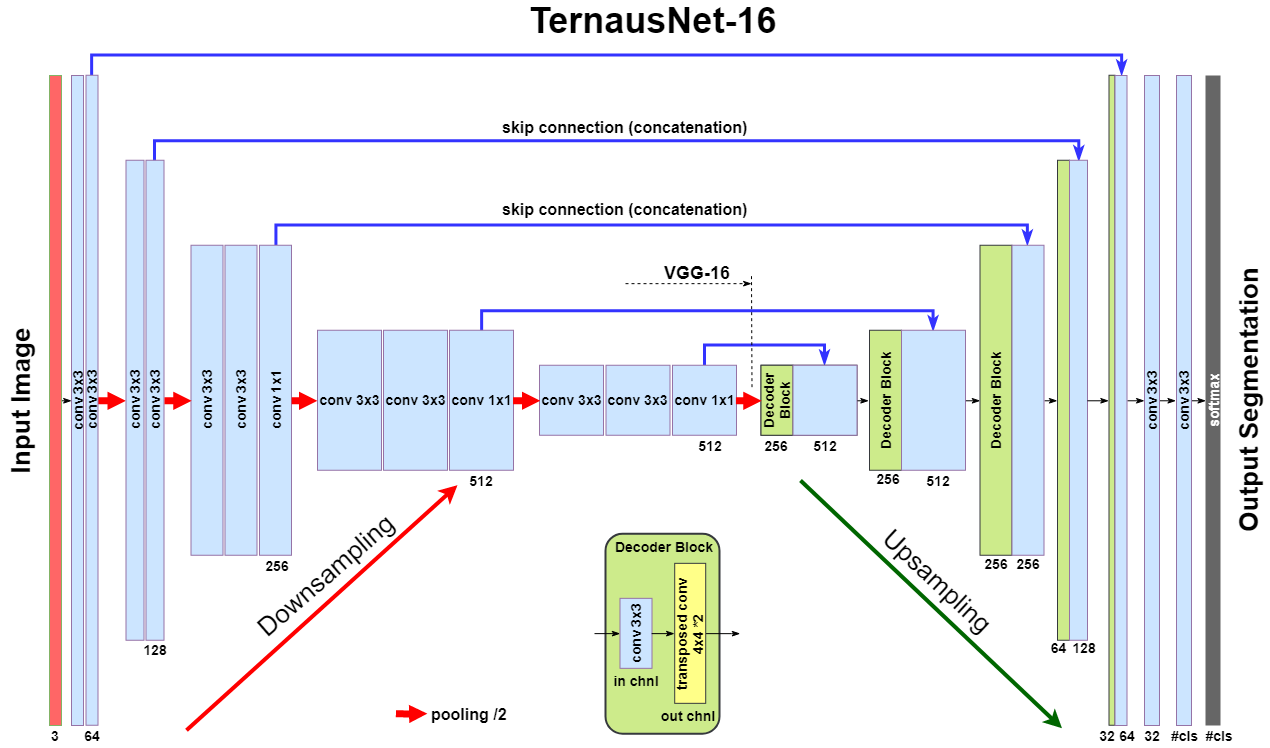
\includegraphics[width=0.8\textwidth]{figure/TernausNet.png}
        \caption{TernausNet结构图}
    \end{figure}
    \item LinkNet-34是另一种对UNet的改进方法,采用了ResNet-34作为encoder。此外在decoder block上也有了改进:添加了batch normalization和1*1的卷积。
    \begin{figure}[H]
        \centering  %图片全局居中
        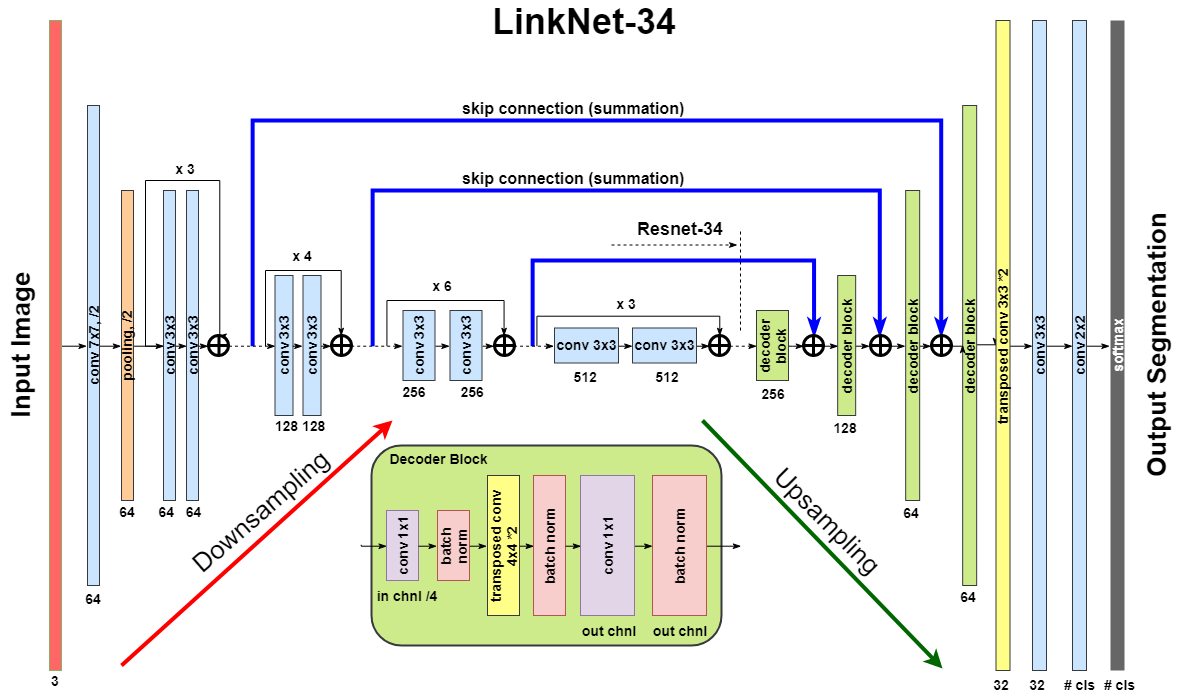
\includegraphics[width=0.8\textwidth]{figure/LinkNet34.png}
        \caption{LinkNet结构图}
    \end{figure}
\end{itemize}

\subsubsection{多任务网络}
此外,由于以上几种网络对instrument类问题的分割效果并不好,因此考虑到各类问题之间的相互关联关系,设计了基于TDSNet% TODO cite2
的多任务网络。

\begin{figure}[H]
    \centering  %图片全局居中
    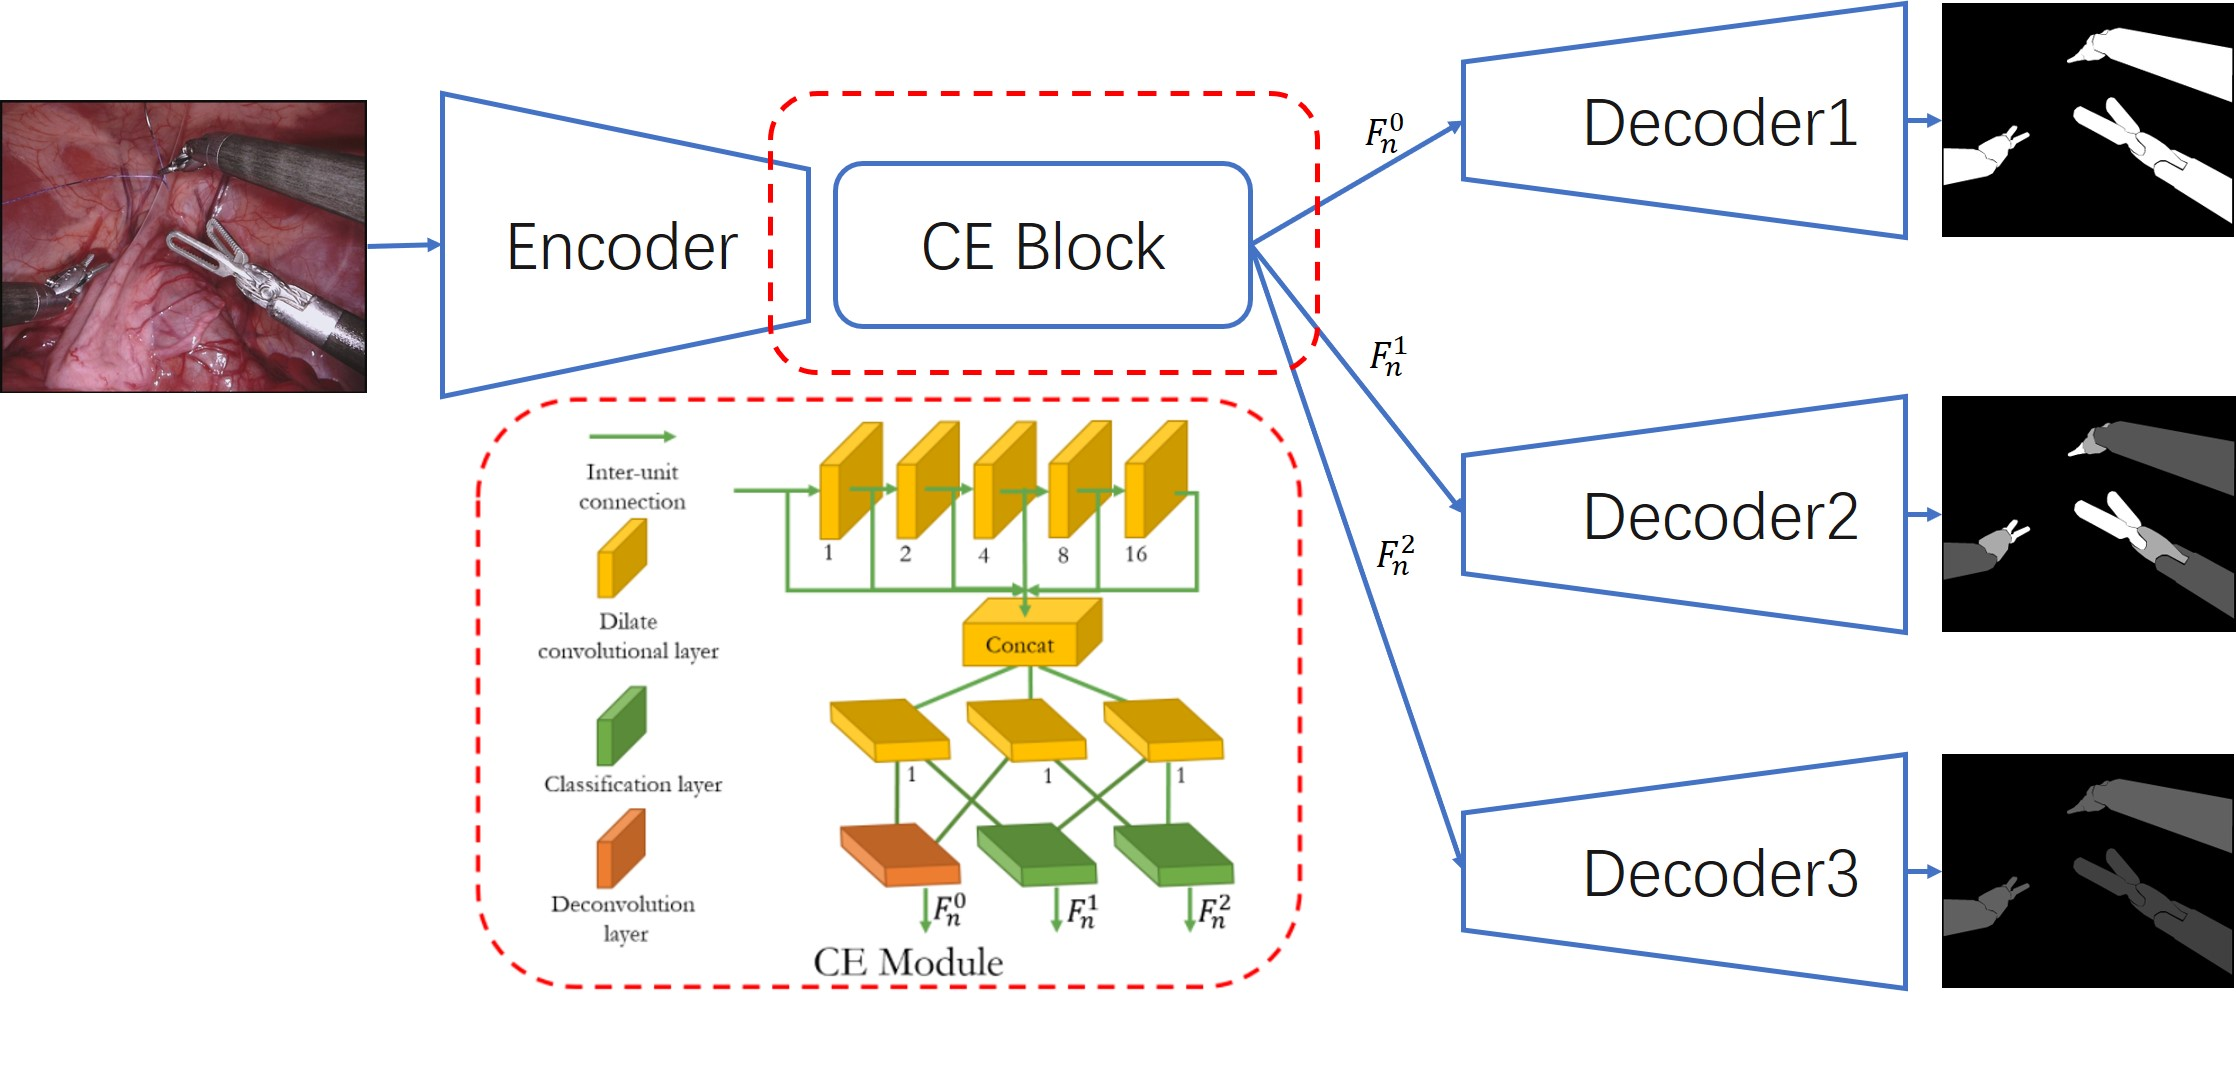
\includegraphics[width=0.8\textwidth]{figure/TDSNet.jpg}
    \caption{TDSNet结构图}
\end{figure}
TDSNet的要点在于在encoder和decoder之间插入了一个CE Block,在这个CE Block中依次使用了不同步长的dilate convolution以整合不同大小的特征。随后将CE Block的输出$F_n^0,F_n^1,F_n^2$输入三个decoder,并对应三种不同的分类任务。这样将三个不同的任务共用一个encoder,在理论上可以避免模型参数过多,并且在重点进行其中一个任务的分割时,可以有效利用到其他两个任务ground truth中所包含的信息,同时也提升了模型的运行速度。

\subsection{训练参数的选取}
\begin{itemize}
    \item 选用$L=H-k\log J$作为损失函数,其中H为交叉熵(cross entropy),k为常数(实际训练时取0.3),J为dice score,可以表示为
    $$J=\frac{1}{n}\sum_{i=1}^n(\frac{y_i\hat{y}_i}{y_i+\hat{y}_i-y_i\hat{y}_i})$$
    在使用TDSNet时,损失函数为三者的加权和,实际使用时binary,parts,instruments三者的权重分别为% TODO
    \item 选用的优化器为Adam
    \item 学习率采用阶梯式,即前10个epoch采用1e-4使其更快收敛,后十个epoch采用1e-5。
    \item 将数据集分为[1, 3],[2, 5],[4, 8] [6, 7]四个fold,每次取其中一组作为valid set其余作为训练集,进行交叉验证算法。
\end{itemize}






\section{结果评估}
\subsection{评价指标的选取}
由于模型的输出和ground truth均为分割后的图像,因此评价指标的选取就比较简单,采用了图像分割中常用的iou和dice作为评价指标。定义预测为阳性的区域为A,ground truth中阳性区域为B,则两者的计算公式如下:

\begin{equation}
    IoU=\frac{|A\cap B|}{|A\cup B|}=\frac{|A\cap B|}{|A|+|B|-|A\cup B|}
\end{equation}

\begin{equation}
    Dice=\frac{2|A\cap B|}{|A|+|B|}
\end{equation}

\subsection{各方法结果对比}


\subsection{模型评价}

\section{感想与展望}
本次大作业是我第一次真正有机会独立完成有关深度学习的项目。在完成项目的时间里,我学习了一些关于深度学习的基本知识,Pytorch框架的使用和一个深度学习项目基本的组成部分。根据老师给的参考资料上的思路,也自己搭建了一个基于TDSNet的神经网络。虽然可能因为一些细节的问题导致效果不佳,但是在完成项目的过程中我还是学到了很多,也算是对深度学习这个热门领域有了入门的了解,并且接触到了实际的科研问题。

最后模型实现的结果没能达到预期还是比较遗憾,但是个人在完成项目的过程中也收获了很多。最后感谢老师和助教在本次项目完成过程中给予我的帮助!


\end{document}
